\chapter{Introdução}

Inteligência artificial é um campo da ciência da computação que estuda
``agentes inteligentes'', que de certa forma percebem o ambiente à sua volta
e tomam ações tendo como objetivo maximizar a chance de sucesso de alguma
tarefa específica. Uma utilização muito comum nos dias de hoje é a de
inteligência artificial com o objetivo de criar um agente capaz de competir
com humanos em jogos com alto nível de estratégia, como Xadrez\footnote{inserir referência
na bibliografia} e Go\footnote{disso também}.
Decidimos então estudar inteligência artificial para a realização deste
trabalho com a ideia de modelar um outro jogo de estratégia,
\textbf{Magic: The Gathering}.

\textit{Magic} foi lançado em 1993, introduzindo o conceito de trading card
game. Com o sucesso do jogo e popularização dos jogos digitais, eventualmente
nasceram versões digitais do jogo para computadores e videogames, e com isso
nasceu a necessidade de agentes que jogassem contra os jogadores. Atualmente
há várias versões digitais de Magic, mas nenhuma tem uma inteligência artificial
boa o suficiente para se provar desafiadora contra jogadores experientes, uma vez
que a cada ação há uma grande quantidade de ações possíveis e elementos como
blefe envolvidos. Nossa intenção é entender a complexidade da representação do
jogo e criar uma plataforma para jogar Magic que possibilite a implementação de
um agente de inteligência artificial.

Na próxima seção iremos introduzir alguns conceitos e regras básicas do jogo,
de modo a possibilitar a familiarização do leitor com \textbf{Magic}, facilitando
a compreensão do restante do trabalho.

\section{Conceitos básicos}

Um jogo usual de \textit{Magic: the Gathering} conta com dois jogadores munidos
de um baralho de 60 cartas cada, ambos começando com 20 pontos de vida, sendo
que o objetivo é reduzir o total de pontos de vida do oponente a 0. Para tanto,
é preciso usar as cartas disponíveis na mão, que podem representar feitiços,
criaturas ou terrenos (existem outros tipos de cartas, mas para nossa implementação
iremos focar nesses três). Feitiços são cartas que têm um efeito que acontece
no momento em que são jogadas e então são colocadas no cemitério (como é chamada
a pilha de descarte no jogo).

\vskip1ex

Por exemplo, o feitiço Divinação tem um efeito simples: "Compre dois
cards" (na versão em português do jogo, as cartas são referenciadas pela palavra
em inglês \textit{cards}). O jogador que joga esta carta pega as duas cartas do
topo de seu baralho e as coloca em sua mão, aumentando o leque de possibilidades.
Assim, \textbf{feitiços} podem alterar o estado do jogo de diversas maneiras
(como fazer com que os jogadores comprem ou descartem cartas, alterar o total de
pontos de vida de um jogador ou destruir uma criatura) e são a principal forma
de interagir com o oponente ou desenvolver o seu lado do campo de batalha (como
é chamada a zona do jogo em que ficam as criaturas e terrenos).

\begin{figure}[!h]
    \centering
    \begin{minipage}{0.45\textwidth}
        \centering
        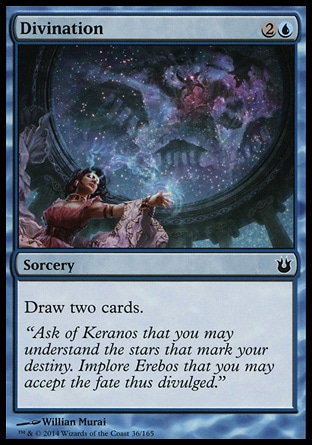
\includegraphics[width=0.5\textwidth]{picstcc/divination.jpg}
        \caption{Divinação (Feitiço)}
        \label{divination}
    \end{minipage}\hfill
    \begin{minipage}{0.45\textwidth}
        \centering
        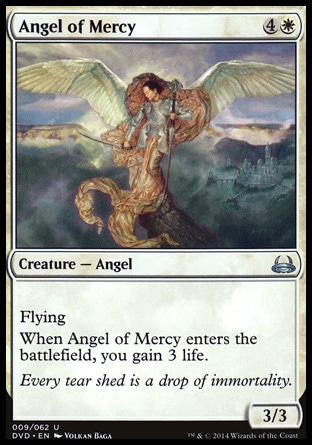
\includegraphics[width=0.5\textwidth]{picstcc/angelOfMercy.jpg}
        \caption{Anjo da Misericórdia (Criatura)}
        \label{anjo}
    \end{minipage}
\end{figure}

\textbf{Criaturas} são cartas permanentes (uma vez jogadas elas
permanecem no campo de batalha até que sejam destruídas por algum
feitiço ou durante o combate) que possuem poder (quantidade de dano
causado em combate), resistência (quantidade de dano necessária para ser
destruída) e muitas vezes habilidades que afetam o andamento do combate
ou que fazem algum efeito no momento em que são jogadas.

\vskip1ex

Por exemplo, Anjo da Misericórdia tem a habilidade de Voar (que limita
as interações do oponente durante o combate) e concede a seu controlador
3 pontos de vida ao entrar no campo de batalha. Além disso, seu poder e
resistência são 3 e 3, respectivamente, conforme indicado na caixa no
canto inferior direito.

\vskip1ex

\textbf{Terrenos} são a fonte de \textit{mana}, que é o recurso utilizado para
pagar por criaturas e feitiços. O custo de \textit{mana} das cartas que não são
terreno está indicado no canto superior direito da carta (por exemplo, para
jogar Divinação é necessário usar três terrenos, sendo que um deles deve ser
necessariamente uma Ilha, como na figura \ref{ilha}). Terrenos são, portanto, um
dos tipos de cartas mais importantes, pois sem eles não há maneira (normalmente)
de jogar suas outras cartas. Uma vez utilizado, um terreno se torna \textbf{virado}
(em inglês, \textit{tapped}): para jogar uma carta que não seja terreno, é
necessário virar o número de terrenos equivalente ao seu custo. Uma vez virado,
o terreno permanece virado até o começo do próximo turno de seu controlador,
quando poderão ser utilizados novamente. Desta maneira, são necessários quatro
terrenos para se jogar duas cartas custando duas manas cada durante o mesmo turno.

\begin{wrapfigure}{R}{5cm}
    \centering
    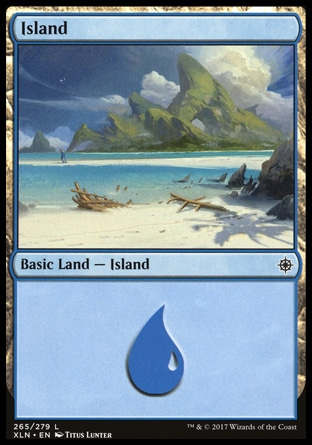
\includegraphics[width=0.25\textwidth]{picstcc/island.jpg}
    \caption{Ilha (Terreno)}
    \label{ilha}
\end{wrapfigure}

Uma parte importante do jogo é o sistema de \textit{cores}. As cartas do jogo
são divididas entre cinco cores de mana, com um terreno associado que produz
mana desta cor: Branco (Planície), Azul (Ilha), Preto (Pântano), Vermelho
(Montanha) e Verde (Floresta). Cada cor tem mecânicas de jogo únicas, fazendo
com que jogadores usem mais de uma cor de mana em seus baralhos para ter acesso
a tipos de efeitos diferentes, ao custo de utilizar terrenos variados, criando
a possibilidade de não ter o terreno certo para jogar a carta desejada.

Para este trabalho utilizaremos apenas baralhos de uma única cor.

\vskip1ex

\section{Estrutura do jogo}
\label{gamestructure}

No começo do jogo é decidido aleatoriamente quem será o jogador inicial,
e então os dois jogadores compram uma mão inicial de sete cartas.
Antes do jogo propriamente dito começar, os jogadores podem optar por tomar uma
ação chamada \textit{mulligan}, que consiste em rejeitar a mão inicial, embaralhá-la
de volta com o restante dos cards e comprar uma nova mão inicial, com uma carta
a menos. Pode-se então repetir o processo até que cada jogador esteja satisfeito
com a mão inicial ou até o jogador realizar um mulligan com apenas uma carta na
mão (resultando em uma mão de zero cartas, onde não há mais a possibilidade de
realizar mulligan). Uma vez que os dois jogadores tiverem escolhido manter uma
mão inicial, cada jogador que realizou pelo menos um mulligan olha a carta do
topo de seu \textit{deck} (como é chamado o baralho) e decide se quer colocá-la
no fundo.

\vskip1ex

O jogo então começa, com os jogadores alternando entre turnos, onde o
jogador que ``controla o turno'' é chamado de \textit{jogador ativo},
com a seguinte estrutura, simplificada:

\begin{itemize}
    \item\textbf{Início do turno}: Permanentes do jogador ativo são
desviradas. Jogador ativo compra uma carta de seu \textit{deck}.
    \item\textbf{Primeira Fase Principal}: Jogador ativo pode jogar as
cartas da mão.
    \item \textbf{Combate}: Jogador ativo ``declara atacantes'' (escolhe
quais de suas criaturas irão atacar seu oponente); em seguida, seu
oponente ``declara bloqueadores'' (escolhe quais de suas criaturas irão
bloquear as criaturas atacantes). Caso alguma criatura atacante esteja bloqueada
por mais de uma criatura, o jogador ativo decide, então, a ordem com que o dano será
atribuído a cada criatura bloqueadora. Por fim, cada criatura não-bloqueada
causa dano igual ao seu poder ao oponente e todas as criaturas
bloqueadas e bloqueadoras causam dano entre si.
    \item \textbf{Segunda Fase Principal}: Igual à primeira Fase
Principal.
\end{itemize}

A estrutura acima se repete até o jogo terminar, o que acontece
geralmente quando algum jogador chega a 0 pontos de vida,
mas também pode acontecer de outras maneiras como, por exemplo, se o
baralho de um jogador acabar.
